\clearpage
\section{Appendix: Training framework}
\label{sec:training_fwk}
This section describes the work which was done at software level which is definitely not a part that can be neglected when working in group on such a complex machine learning project (a lot of heavy computation power required, long training times for limited chances for improvements).  We describe the constraints we had to face and the solutions we found to overcome them. We trained nearly a hundred experiments which requires good organization and a way to track and monitor everything.
We came out with a convenient solution which allows respecting all the project constraints and allowed us to focus on the machine learning part of the project.

\subsection*{Constraints statement}
\label{sec:Constraints}
As this work was to  be done in group, we have to develop a framework so everyone could work and share their code independently.
\begin{itemize}
    \item Heterogeneous environments: several operating systems (linux, windows, macOS), various platforms (local laptop training, Kaggle Kernels notebook, remote machines at Ecole Polytechnique). On every platform, data has to be acessible and experiments results have to be stored in a way they can be retrieved. We used the Kaggle dataset feature to  host the raw dataset as well as the preprocessed data.
    \item Privacy: as not sharing code was among the rules of the challenge, our source code remained private on GitHub (\textit{which made cloning operations even trickier when using Kaggle kernels}).
    \item Reproducibility: all our experiments are reproducible (source code tracking under git, local and cloud storage of experiments results using ~\href{https://wandb.ai/molecule-nlp-altegrad-23/molecule-nlp}{Weights and biases}).
    \item Cost: project total budget limit to 50euros. \textit{Google Collab would not have met this requirements considering the amount of experiments we did and the long training times}.
\end{itemize}


We wrote a framework which takes and solves all these constraints at once and allows to focus on training models.

\subsection*{Definition of an experiment}
An experiment is defined by a unique identifier and the instantiation of a model (tokenization method, architecture of the LLM and GNN), the configuration of an  optimizer and training hyper parameters. At inference time, we're using this unique identifier so we can safely instantiate a network and reload the weights (\textit{trained model are by construction compatible with inference. This avoids the risk of having a `.pth` weight file without knowing which architecture to use to reload it.}).
Launching the training of an experiment goes seamlessly with the following command line, below is the example for experiment 620:
\begin{verbatim}
    python train.py -e 620
\end{verbatim}

The same exact training can be ran directly on Kaggle using their API.
\begin{verbatim}
    python remote_training.py -e 620 -p -nb mol-nlp
\end{verbatim}
Finally, the evaluation mechanism generates the submission csv file and the right Kaggle API command line which can be used to submit to the hosted challenge (with a message which allows to know exactly which experiment was submitted in which conditions).

\begin{verbatim}
python evaluation.py -e 620
\end{verbatim}

\begin{figure}
    \centering
    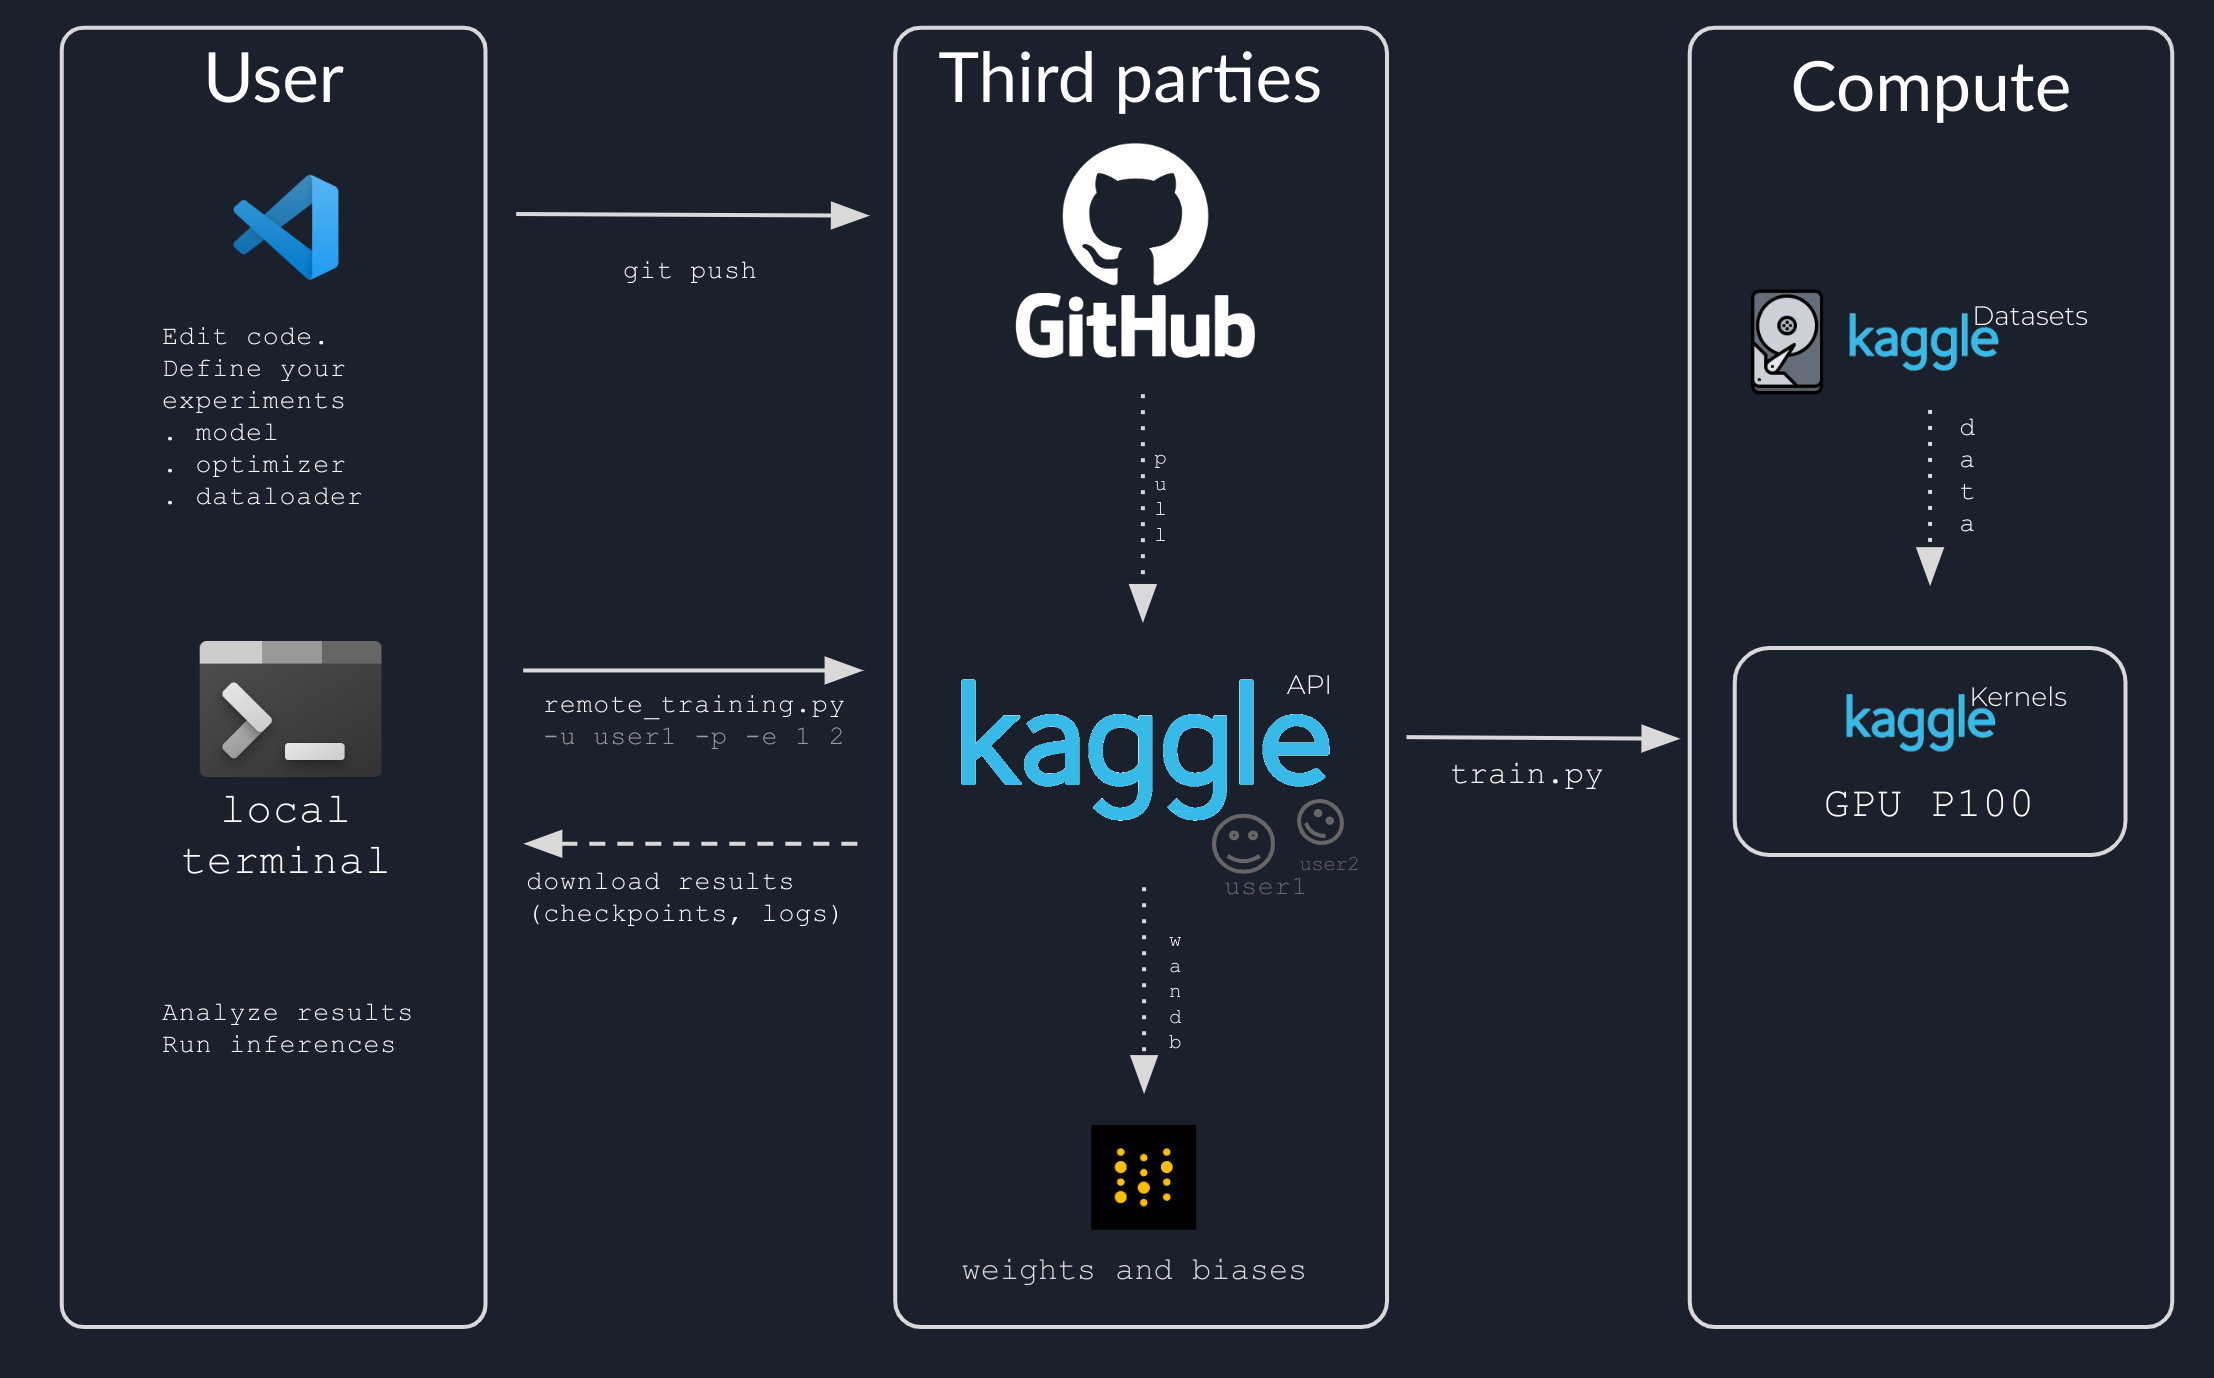
\includegraphics[width=0.5\textwidth]{figures/training_framework.png}
    \caption{Remote training framework allows accessing free GPU resources on Kaggle Kernels. Local code is synchronized through our \textbf{private Github repository} (until the 4th of February) so the remote notebook can be run with the same code. The \textbf{Kaggle dataset} feature is used to store the raw dataset and the preprocessed data (for each tokenizer, we have stored the preprocessed dataset which saves nearly 10 minutes of computation time at the begining of each experiment). To fine tune our own models, we use \href{https://huggingface.co/balthou}{Hugging Face} as an exchange platform so we could easily start from a checkpoint from any remove computer. The \textbf{Weights and biases} platform is used to track the experiments results and monitor the training. Once finished, trained models can be retrieved by pulling the results.
    Note that the small piece of code to help access Kaggle notebooks freely from the terminal was made available \href{https://github.com/balthazarneveu/mva\_pepites}{publicly} (totally independantly from this challenge) to be later used on other projects.
    }
    \label{fig:training_framework_schema}
\end{figure}

\subsection*{Training conditions}
\label{sec:training conditions}

\begin{table*}[ht]
    \centering
    \begin{tabular}{lcccc}
    \hline
    \textbf{Feature} & \textbf{Nvidia T500} & \textbf{Nvidia RTX 2060} & \textbf{Nvidia K100} & \textbf{Nvidia A4000} \\ \hline
    OS & Linux & Linux WSL & Linux in Docker & Linux \\  
    Location            & local laptop           & local laptop  & Kaggle  & Ecole Polytechnique  \\
    Access & direct & direct & Kaggle Kernels & SSH \\
    Dataset access & local SSD & local SSD & Kaggle dataset & remote download + SSD drives\\ 
    Memory           & 4 GB                        & 6 GB                           & 16 GB                          & 24 GB                          \\
    Student cost & - & Electricity $\approx$ +20 euros/month & Free & Free \\
    Availability & $\infty$ & $\infty$ & 30 hours/week 12hours/experiment & $\approx \infty$ weekends and night \\
    \hline
    \end{tabular}
    \caption{Comparison of the training platform and GPUs which were used during training}
    \label{table:gpu_comparison}
\end{table*}


To setup the training loop, we started on a single NVIDIA GeForce RTX T500 local GPU with 4Gb of RAM (\textit{the baseline provided by the challenge organizers did not even run because of memory limitation}). This was enough to make sure we could train, track and monitor progress of all our experiments and build a whole local training framework. We started by freezing the LLM weights to reduce the amount of memory required and get decent batch sizes even on the tiny T500 GPU. Due to low performances, the need to access bigger computation resources quickly came so we had to overcome this difficulty by making our framework agnostic to the training platform and still be able to recover our results and monitor from anywhere. The diversity of training and hardware platforms is shown in \ref*{table:gpu_comparison}. We considered using Google Colab Pro (datasets and models shared through Google drive) but with the consideration that we have long training times, the cost would have been prohibitive. We found a good compromise and did many experiments using Kaggle Kernels through the API which are free and provide GPU access with 16Gb of RAM during a maximum time of 12 hours per session and up to 30hours per week.
